% % % %
% % % % Solution
% % % %
\section{Solution}

\begin{frame}\frametitle{Domain knowledge: diabetic retinopathy symptoms}

\begin{itemize}
\item {\hyperlink{https://goo.gl/s5lMt8}{DR symptoms cheatsheet: https://goo.gl/s5lMt8}
\begin{center}
\par 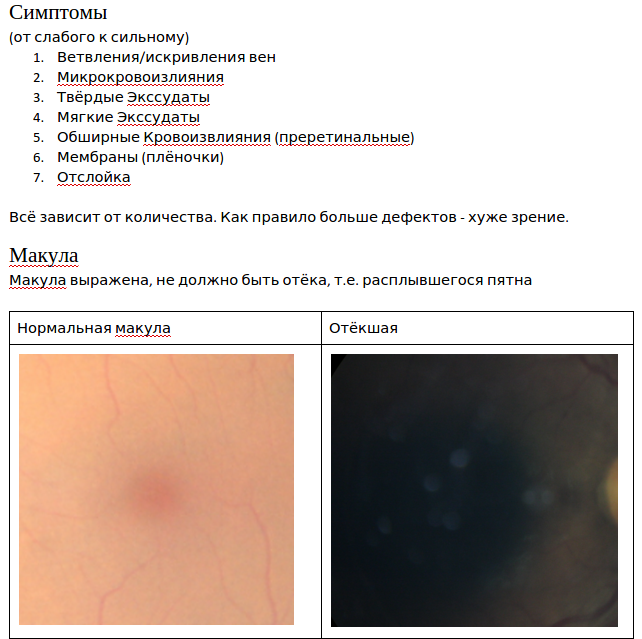
\includegraphics[interpolate=true,valign=c,width=0.4\textwidth]{pics/symptoms_pic.png}
\end{center}
Was prepared with assistance of Vera Shevchenko
}
\item \href{http://www.icoph.org/downloads/Diabetic-Retinopathy-Detail.pdf}{International Clinical Diabetic Retinopathy Disease Severity Scale, Detailed Table: \small http://www.icoph.org/downloads/Diabetic-Retinopathy-Detail.pdf}
\end{itemize}

\end{frame}

\subsection{Data preparation}


\begin{frame}\frametitle{Preprocessing}
\begin{columns}

\begin{column}{9cm}
\begin{itemize}
\item Crop black borders
\vspace{20pt}

\item Extent to square + resize
\vspace{20pt}

\item Optionally: crop internal square
\vspace{20pt}

\item Optionally: Local Contrast Normalization (LCN) \\ 
      $ \hat{I}_{x,y} = \frac{I_{x,y} - \mu_{x,y}}{\sigma_{x,y}} $
\end{itemize}
\end{column}

\begin{column}{6cm}
\begin{tabular}{ @{}c m{0.25cm} c }

	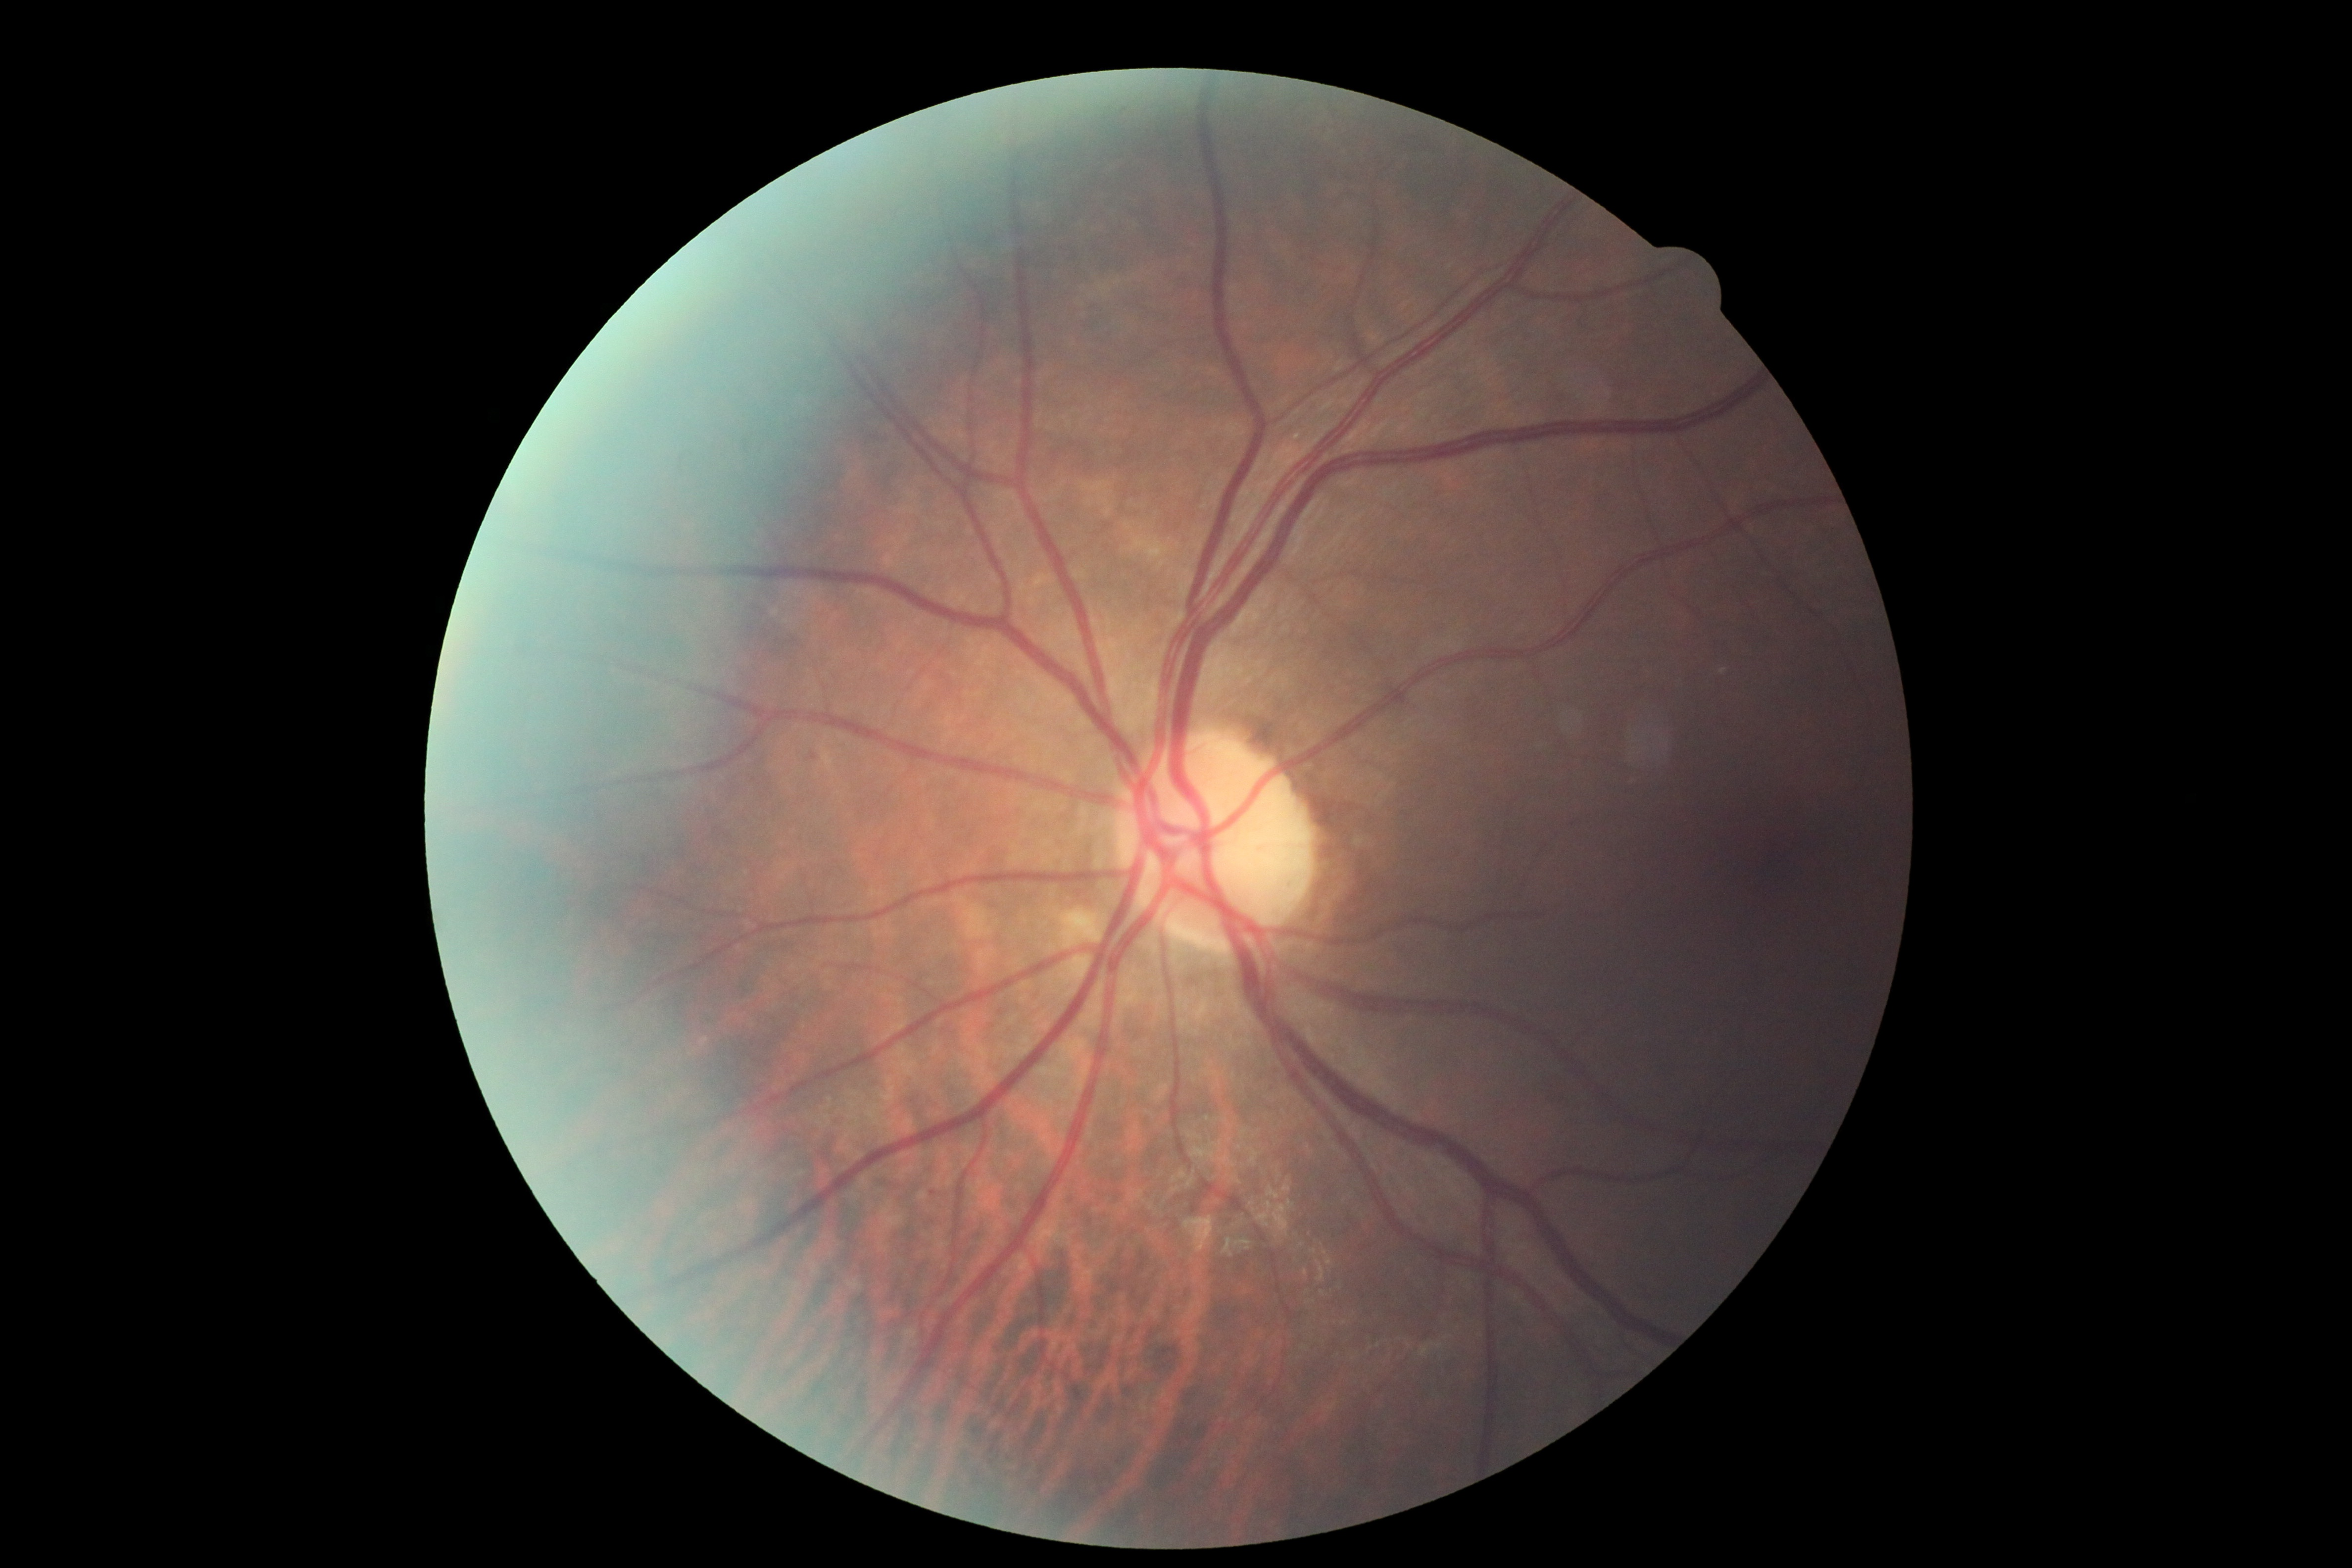
\includegraphics[valign=c,height=0.5cm]{pics/10_left.jpeg} & $\rightarrow$ &
    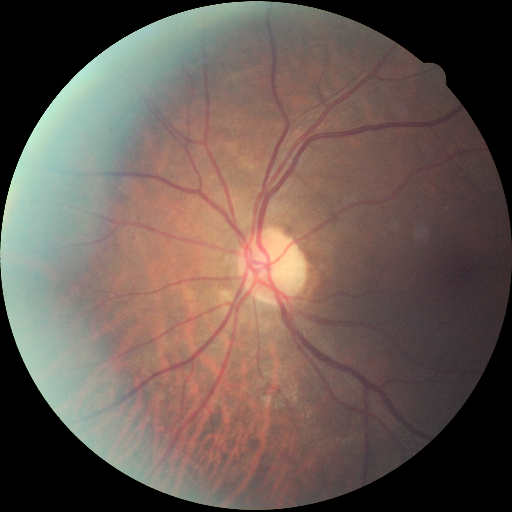
\includegraphics[valign=c,height=0.5cm]{pics/10_left.png}
    \vspace{10pt} \\ 
    
	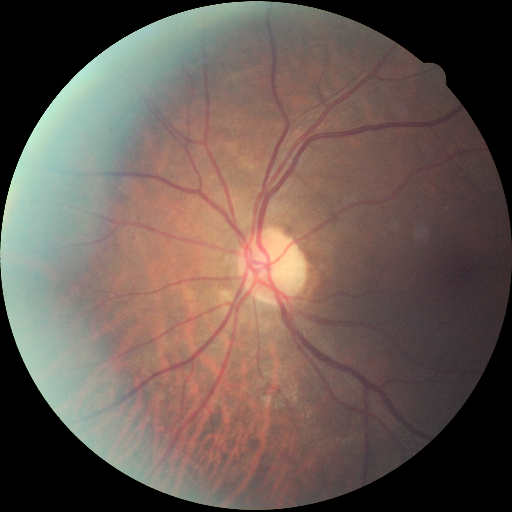
\includegraphics[valign=c,height=0.5cm]{pics/10_left.png} & $\rightarrow$ &
    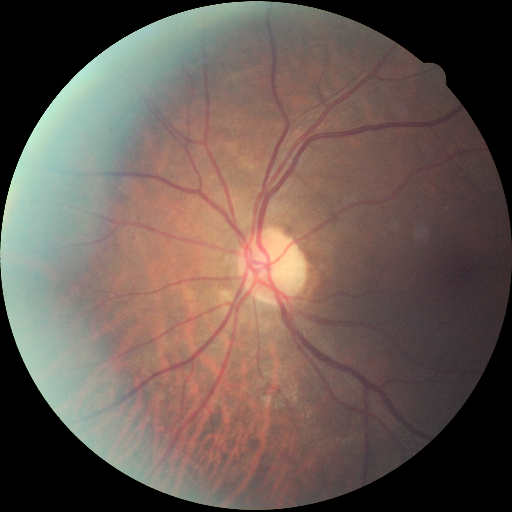
\includegraphics[valign=c,height=0.25cm]{pics/10_left.png}
	\vspace{10pt} \\ 	

	\adjustbox{valign=c}{\begin{tikzpicture}
	    \node[anchor=south west,inner sep=0] (image) at (0,0) {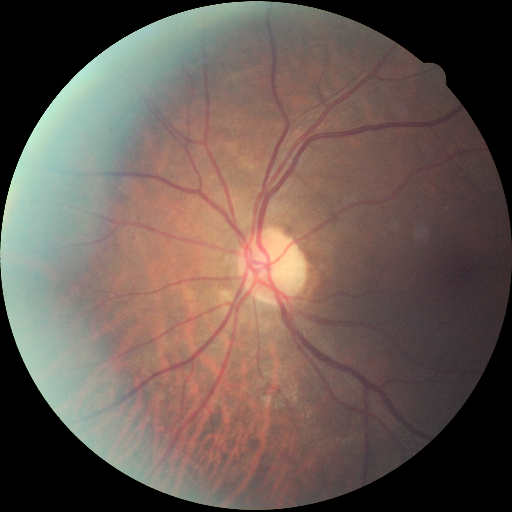
\includegraphics[valign=c,height=0.5cm]{pics/10_left.png}};
	        \begin{scope}[x={(image.south east)},y={(image.north west)}]
	            \draw[red] (0,0.5) -- (0.5,1) -- (1,0.5) -- (0.5,0) -- (0,0.5);
	        \end{scope}
	\end{tikzpicture}} & $\rightarrow$ &
	    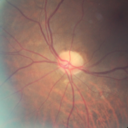
\includegraphics[valign=c,height=0.5cm]{pics/10_left_inner.png}
    \vspace{10pt} \\

%    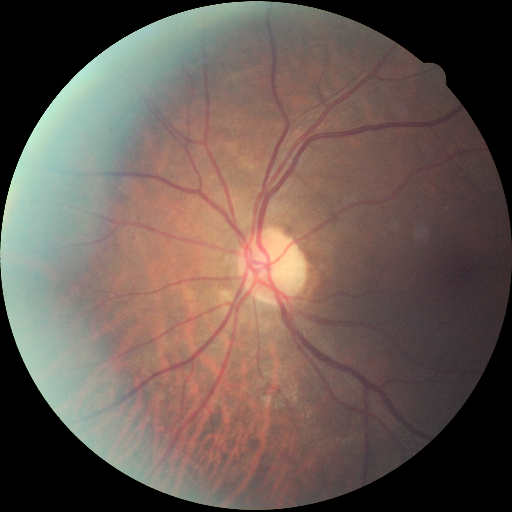
\includegraphics[valign=c,height=0.5cm]{pics/10_left.png} & $\rightarrow$ &
%    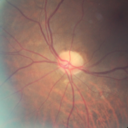
\includegraphics[valign=c,height=0.5cm]{pics/10_left_inner.png}
%	\vspace{10pt} \\

	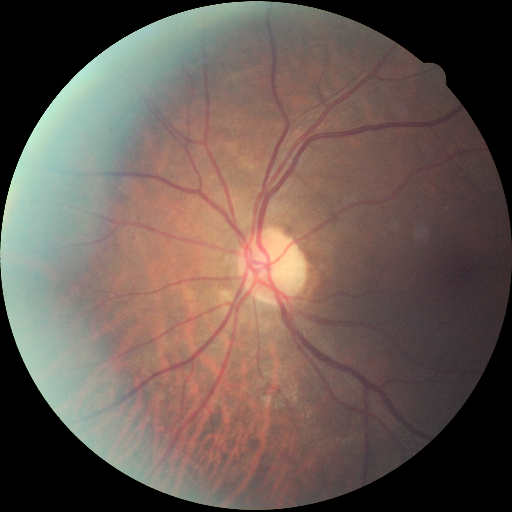
\includegraphics[valign=c,height=0.5cm]{pics/10_left.png} & $\rightarrow$ &
	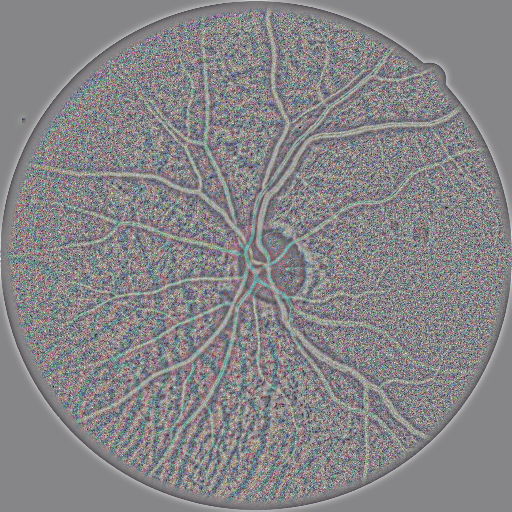
\includegraphics[valign=c,height=0.5cm]{pics/10_left_lcn.png}
	\\


\end{tabular}
\end{column}

\end{columns}
\end{frame}

\begin{frame}\frametitle{Augmentation}
\begin{itemize}
\item Random mirror
\item Random rotation
\item Color augmentation - not helped
\end{itemize}

\end{frame}

\subsection{Network configuration}
\begin{frame}\frametitle{}
\par Slice rotate
\par Merge
\par Output
\end{frame}

\begin{frame}\frametitle{Network configuration}
\centering
\begin{table}[]
\tiny
\centering
\begin{tabular}{@{}clcllr@{}}
\toprule
   & Layer type                & Size &             & Output Shape        & Outputs \\ \midrule
1  & InputLayer                &      &             & (64, 3, 256, 256)   & $196\,608$  \\
2  & \textbf{SliceRotateLayer} &      &             & (256, 3, 128, 128)  & $49\,152$   \\
3  & Conv2DDNNLayer            & 3x3  & LReLU       & (256, 64, 126, 126) & $1\,016\,064$ \\
4  & MaxPool2DDNNLayer         & 3x3  & stride 2x2  & (256, 64, 62, 62)   & $246\,016$  \\
5  & DropoutLayer              &      & P=0.1       & (256, 64, 62, 62)   & $246\,016$  \\
6  & Conv2DDNNLayer            & 3x3  &             & (256, 96, 60, 60)   & $345\,600$  \\
7  & MaxPool2DDNNLayer         & 3x3  & stride 2x2  & (256, 96, 29, 29)   & $80\,736$   \\
8  & DropoutLayer              &      & P=0.2       & (256, 96, 29, 29)   & $80\,736$   \\
9  & Conv2DDNNLayer            & 3x3  & LReLU       & (256, 128, 27, 27)  & $93\,312$   \\
10 & DropoutLayer              &      & P=0.3       & (256, 128, 27, 27)  & $93\,312$   \\
11 & Conv2DDNNLayer            & 3x3  & LReLU       & (256, 96, 25, 25)   & $60\,000$   \\
12 & MaxPool2DDNNLayer         & 3x3  & stride 2x2  & (256, 96, 12, 12)   & $13\,824$   \\
13 & DropoutLayer              &      & P=0.4       & (256, 96, 12, 12)   & $13\,824$   \\
14 & Conv2DDNNLayer            & 3x3  & LReLU       & (256, 128, 10, 10)  & $12\,800$   \\
15 & MaxPool2DDNNLayer         & 2x2  & stride 2x2  & (256, 128, 5, 5)    & $3\,200$    \\
16 & \textbf{RotateMergeLayer} &      &             & (64, 12800)         & $12\,800$   \\
17 & DropoutLayer              &      & P=0.5       & (64, 12800)         & $12\,800$   \\
18 & DenseLayer                & 512  &             & (64, 512)           & $512$     \\
19 & FeaturePoolLayer          &      & FeaturePool & (64, 256)           & $256$     \\
20 & DropoutLayer              &      & P=0.5       & (64, 256)           & $256$     \\
21 & DenseLayer                & 512  &             & (64, 512)           & $512$     \\
22 & FeaturePoolLayer          &      & FeaturePool & (64, 256)           & $256$     \\
23 & DropoutLayer              &      & P=0.5       & (64, 256)           & $256$     \\
24 & DenseLayer                &      &             & (64, 4)             & $4$       \\ \bottomrule
\end{tabular}
\end{table}

\end{frame}


\begin{frame}\frametitle{Special layers}

\begin{columns}[t]
\begin{column}{5cm}
\centering
\par SliceRotateLayer

\vspace{0.25cm}

\begin{tikzpicture}[auto, node distance=0.1cm, >=latex]
	\node[anchor=south west,inner sep=0] (image) at (0,0) {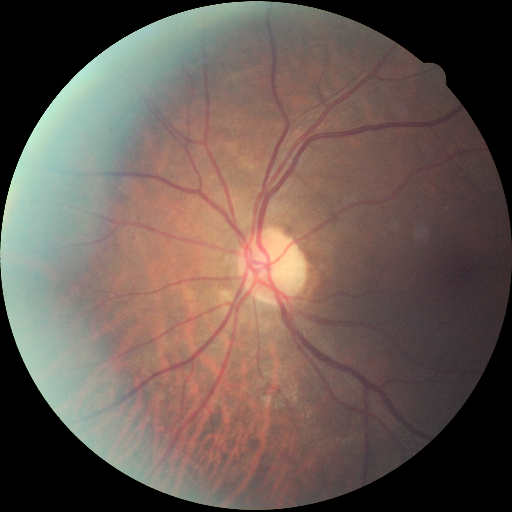
\includegraphics[valign=c,height=1.0cm]{pics/10_left.png}};
	\begin{scope}[x={(image.south east)},y={(image.north west)}]
		\draw[orange,line width=0.4mm] (0,0.51)    rectangle (0.49,1);
		\draw[blue,line width=0.4mm]   (0.51,0)    rectangle (1,0.49);
		\draw[red,line width=0.4mm]    (0,0)       rectangle (0.49,0.49);
		\draw[green,line width=0.4mm]  (0.51,0.51) rectangle (1,1);
	\end{scope}

\end{tikzpicture}

\par $\Downarrow$

\begin{tikzpicture}
% Layers
\begin{scope}[x={(90:1cm)}, y={(0:1cm)}, z={(30:0.15cm)}]
\node[canvas is yx plane at z=0,transform shape] (imageone) at (0,0) {
	\adjincludegraphics[height=1.0cm,trim={0 {.5\width} {.5\width} 0},clip,angle=270,cfbox=blue 1pt 1pt]{pics/10_left.png}};
\node[canvas is yx plane at z=2,transform shape] at (0,0) {
	\adjincludegraphics[height=1.0cm,trim={{.5\width} {.5\width} 0 0},clip,angle=0,cfbox=green 1pt 1pt]{pics/10_left.png}};
\node[canvas is yx plane at z=4,transform shape] at (0,0) {
	\adjincludegraphics[height=1.0cm,trim={{.5\width} 0 0 {.5\width}},clip,angle=90,cfbox=orange 1pt 1pt]{pics/10_left.png}};
\node[canvas is yx plane at z=6,transform shape] at (0,0) {
	\adjincludegraphics[height=1.0cm,trim={0 0 {.5\width} {.5\width}},clip,angle=180,cfbox=red 1pt 1pt]{pics/10_left.png}};
\end{scope}
\end{tikzpicture}



\end{column}
\begin{column}{5cm}
\centering
\par RotateMergeLayer

\begin{tikzpicture}
% Layers
\begin{scope}[x={(90:1cm)}, y={(0:1cm)}, z={(30:0.15cm)}]
\node[canvas is yx plane at z=0,transform shape] (imageone) at (0,0) {
	\adjincludegraphics[height=1.0cm,trim={0 {.5\width} {.5\width} 0},clip,angle=270,cfbox=blue 1pt 1pt]{pics/10_left_cnn.png}};
\node[canvas is yx plane at z=2,transform shape] at (0,0) {
	\adjincludegraphics[height=1.0cm,trim={{.5\width} {.5\width} 0 0},clip,angle=0,cfbox=green 1pt 1pt]{pics/10_left_cnn.png}};
\node[canvas is yx plane at z=4,transform shape] at (0,0) {
	\adjincludegraphics[height=1.0cm,trim={{.5\width} 0 0 {.5\width}},clip,angle=90,cfbox=orange 1pt 1pt]{pics/10_left_cnn.png}};
\node[canvas is yx plane at z=6,transform shape] at (0,0) {
	\adjincludegraphics[height=1.0cm,trim={0 0 {.5\width} {.5\width}},clip,angle=180,cfbox=red 1pt 1pt]{pics/10_left_cnn.png}};
\end{scope}
\end{tikzpicture}

\par $\Downarrow$

%\begin{tikzpicture}[auto, node distance=0.1cm, >=latex]
\par \small Dense layer
\begin{tikzpicture}
\draw [fill=blue]   (0,0) rectangle (1,0.2);
\draw [fill=green] (1,0) rectangle (2,0.2);
\draw [fill=orange]   (2,0) rectangle (3,0.2);
\draw [fill=red] (3,0) rectangle (4,0.2);
\end{tikzpicture}


\end{column}
\end{columns}

\end{frame}

\subsection{Activations}

\begin{frame}\frametitle{}
\begin{center}
%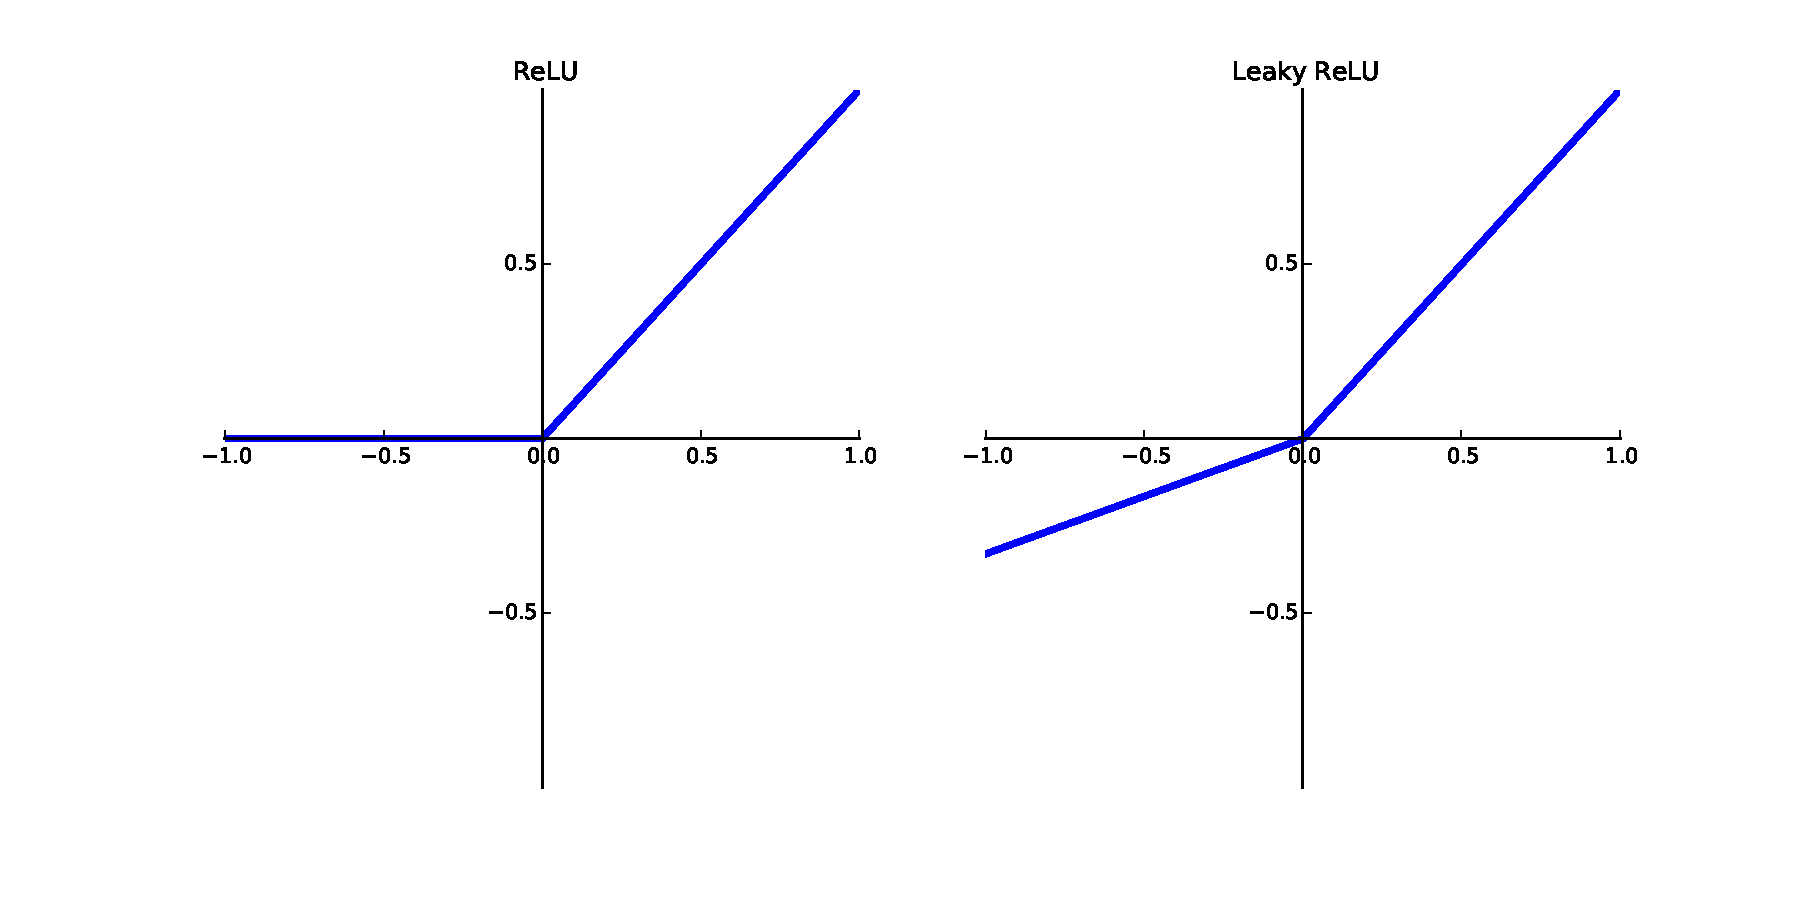
\includegraphics[valign=t,scale=0.25]{pics/relus.pdf}
\end{center}
\par We used Leaky ReLUs for convolutional layer, this activation function acts like a regularizer.
\par Used Maxout\footnote{\href{http://arxiv.org/abs/1302.4389v4}{Maxout Networks. http://arxiv.org/abs/1302.4389v4}} activations for fully-connected layers.
\end{frame}

\subsection{Ordinal regression}

\begin{frame}\frametitle{}
\begin{itemize}

\item Ordinal regression\footnote{\href{https://web.missouri.edu/~zwyw6/files/rank.pdf}{A Neural Network Approach to Ordinal Regression}} is like an ordered classification.
\item Target coding: \\\vspace{0.25cm}
0 $\rightarrow$  0 0 0 0\\
2 $\rightarrow$  1 1 0 0\\
4 $\rightarrow$  1 1 1 1\\
\item Do not normalize the sigmoids in the last fully-connected layer:\\\vspace{0.5cm}
\begin{center}
\begin{Large}
$\frac{e^{-z_i}}{\sum\limits_{i=1}^Ke^{-z_i}}$ $\rightarrow$ $\frac{1}{1 + e^{-z_i}}$
\end{Large}
\end{center}
\end{itemize}
\end{frame}


\subsection{Decision making}

\begin{frame}\frametitle{}
\par Predict score for eyes independently
\par Final score = max(left, right)
\end{frame}


\section{Microaneurysm detection}

\subsection{Motivation}
\begin{frame}\frametitle{Motivation I}

\par Microaneurysms are early symptoms of diabetic retinopathy
\vspace{-20pt}

\begin{table}[]
\begin{tabular}{|p{2cm}|p{8cm}|}
\hline
Disease level &  Findings observable upon dilated ophthalmoscopy \\ \hline
\footnotesize None &  No abnormalities \\ \hline
\footnotesize Mild NPDR & { Microaneurysms only} \\ \hline
\footnotesize Moderate NDPR &  More than just MA but less than severe NPDR \\ \hline
\multirow{4}{*}{\footnotesize Severe NPDR} & \multirow{4}{*}{\begin{tabular}[c]{@{}l@{}}
 $>$20 intraretinal hemorrhages in each quad \\
or  Definite venous beading in 2+ quads \\
or  Intraretinal microvascular anomalies in 1+ quad \end{tabular}} \\
 &  \\
 &  \\
 &  \\ \hline
\footnotesize PDR & \begin{tabular}[c]{@{}l@{}} Neovascularization\\  or/and Vitreous/preretinal hemorrhage\end{tabular} \\ \hline
\end{tabular}
\end{table}

\par \href{http://www.icoph.org/downloads/Diabetic-Retinopathy-Detail.pdf}{\footnotesize International Clinical Diabetic Retinopathy Disease Severity Scale, Detailed Table:  http://www.icoph.org/downloads/Diabetic-Retinopathy-Detail.pdf}

\end{frame}

\begin{frame}\frametitle{Motivation II}
\par We have problems with detection of early symptoms
\par
\begin{figure}
\begin{center}
\vspace{-10pt}
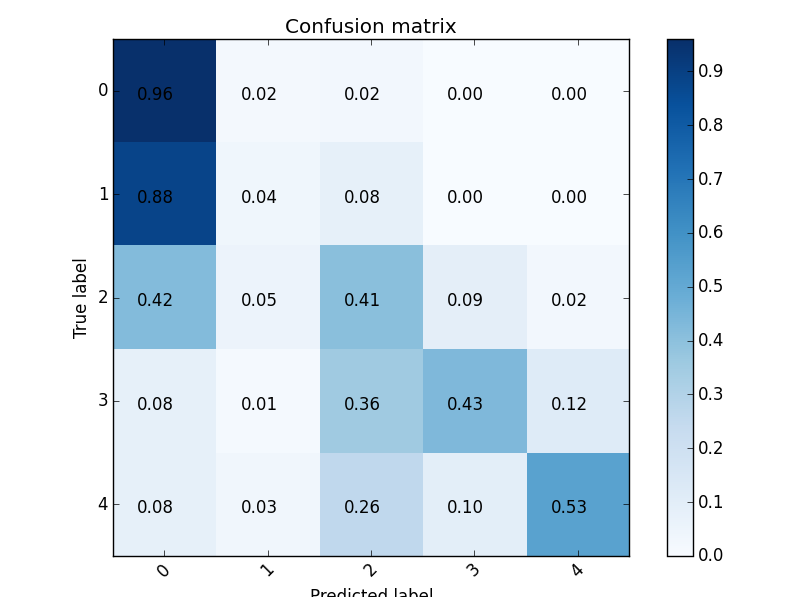
\includegraphics[width=0.4\textwidth]{pics/submission_21_inner_squares_conv5_maxout.png}
\caption{Confusion matrix on 128x128 pixels input}
\vspace{-15pt}
\end{center}
\end{figure}

\par MA have round shape with 2-5 pixels in radius on 1024x1024 image 
\par MA became invisible after downsampling to 128x128/256x256
\par $\Rightarrow$ Classes 0,1,2 almost indistinguishable due to low resolution
\par We have not enough resources\&data to learn on highres images
\par $\Rightarrow$ Let's try plain old image processing

\end{frame}

\subsection{Hessian blob detector} 
\small

\begin{frame}\frametitle{Microaneurysm candidates using the determinant of the Hessian I}

We want to know how much pixel location is similar to blob shape. Let's calculate Hessian matrix at that point:

\[
H(\mathbf{x}) = 
\begin{bmatrix}
L_{xx}(\mathbf{x}) & L_{xy}(\mathbf{x})\\
L_{xy}(\mathbf{x}) & L_{yy}(\mathbf{x})\\
\end{bmatrix}
\]

\begin{itemize}
\item $L_{aa}(\mathbf{x})$ is second partial derivative in the $a$ direction 
\item $L_{ab}(\mathbf{x})$ is the mixed partial second derivative in the $a$ and $b$ directions.
\end{itemize}

\par Derivatives are computed in some scale $\sigma_I$ -- smoothed by a Gaussian kernel
 \[L(\mathbf{x}) = g(\sigma_I) \otimes I(\mathbf{x}) .\]

\par Derivatives must be scaled by factor related to the Gaussian kernel: $\sigma_I^2$.

\end{frame}

\begin{frame}\frametitle{Microaneurysm candidates using the determinant of the Hessian II}

\par At each scale, \textbf{blobs points} are those points that are local extrema of determinant the Hessian matrix. 

\[ \operatorname{det} H(x; \sigma) = \sigma_I^2 ( L_{xx}L_{yy}(\mathbf{x}) - L_{xy}^2(\mathbf{x})) \]

\par Sign of the trace of Hessian matrix help distinguish dark from light points:
\[ \operatorname{trace} H(x; \sigma) = \sigma_I (L_{xx} + L_{yy}). \]

\par Straightforward differential blob detector with automatic scale selection:

\[ 
	(\hat{x}, \hat{\sigma}) = 
	\operatorname{argmaxlocal}_{(x; t)} ( \operatorname{det} H(x; \sigma) ) 
\]

\end{frame}

\newcommand{\includehessiangraphics}[1]{
	\adjincludegraphics[width=0.125\textwidth,trim={{.4\width} {.4\width} {.4\width} {.4\width}},clip]{#1}
}


\begin{frame}\frametitle{Microaneurysm candidates}

\begin{columns}
\begin{column}{1cm}

	\centering

	\par 687\_right

	\adjincludegraphics[width=1.5cm,trim={{.4\width} {.4\width} {.4\width} {.4\width}},clip]{pics/classified_samples/687_right_3.jpg}

	\adjincludegraphics[width=1.5cm,trim={{.4\width} {.4\width} {.4\width} {.4\width}},clip]{pics/classified_samples/687_right_3_high_contrast.jpg}

\end{column}
\begin{column}{11cm}


\begin{tabular}[ht]{ >{\centering\bfseries}m{2cm} @{}c@{}@{}c@{}@{}c@{}@{}c@{}@{}c@{}}
\toprule
 & $\sigma = 1.7$ & $\sigma = 3.4$ & $\sigma =  5.1$ & $\sigma = 6.8$ & $\sigma = 8.0$ \\
\midrule
$L_{xx}$ & 
	\includehessiangraphics{{pics/det_hessian/Lxx_3_000000}.png} &
	\includehessiangraphics{{pics/det_hessian/Lxx_7_000000}.png} &	\includehessiangraphics{{pics/det_hessian/Lxx_15_000000}.png} &	\includehessiangraphics{{pics/det_hessian/Lxx_21_000000}.png} &	\includehessiangraphics{{pics/det_hessian/Lxx_31_000000}.png} \\

$L_{xy}$ &
	\includehessiangraphics{{pics/det_hessian/Lxy_3_000000}.png} &
	\includehessiangraphics{{pics/det_hessian/Lxy_7_000000}.png} &	\includehessiangraphics{{pics/det_hessian/Lxy_15_000000}.png} &	\includehessiangraphics{{pics/det_hessian/Lxy_21_000000}.png} &	\includehessiangraphics{{pics/det_hessian/Lxy_31_000000}.png} \\
	
$L_{yy}$ &
	\includehessiangraphics{{pics/det_hessian/Lyy_3_000000}.png} &
	\includehessiangraphics{{pics/det_hessian/Lyy_7_000000}.png} &	\includehessiangraphics{{pics/det_hessian/Lyy_15_000000}.png} &	\includehessiangraphics{{pics/det_hessian/Lyy_21_000000}.png} &	\includehessiangraphics{{pics/det_hessian/Lyy_31_000000}.png} \\

$\operatorname{det} H(x; \sigma)$ & 
	\includehessiangraphics{{pics/det_hessian/DH_3_000000}.png} &
	\includehessiangraphics{{pics/det_hessian/DH_7_000000}.png} &	\includehessiangraphics{{pics/det_hessian/DH_15_000000}.png} &	\includehessiangraphics{{pics/det_hessian/DH_21_000000}.png} &	\includehessiangraphics{{pics/det_hessian/DH_31_000000}.png} \\
\bottomrule
\end{tabular}

\end{column}
\end{columns}


\end{frame}

\begin{frame}\frametitle{Microaneurysm candidates}
\centering
\only<1>{
\begin{tabular}{|@{}c@{}|@{}c@{}|@{}c@{}|@{}c@{}|@{}c@{}|}
\hline

Normal & Mild & Moderate & Severe & Proliferative \\

\hline
	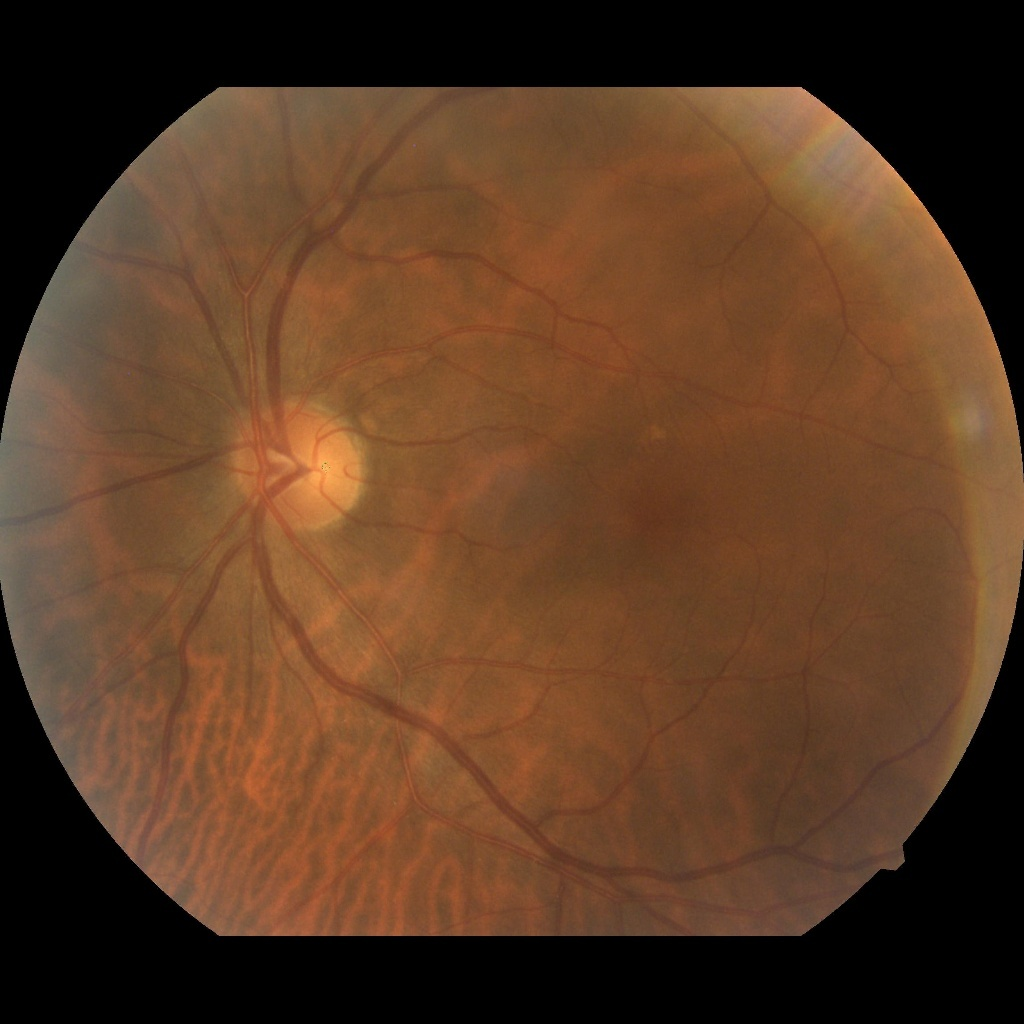
\includegraphics[width=0.2\textwidth]{pics/classified_samples/197_left_0.jpg} &
	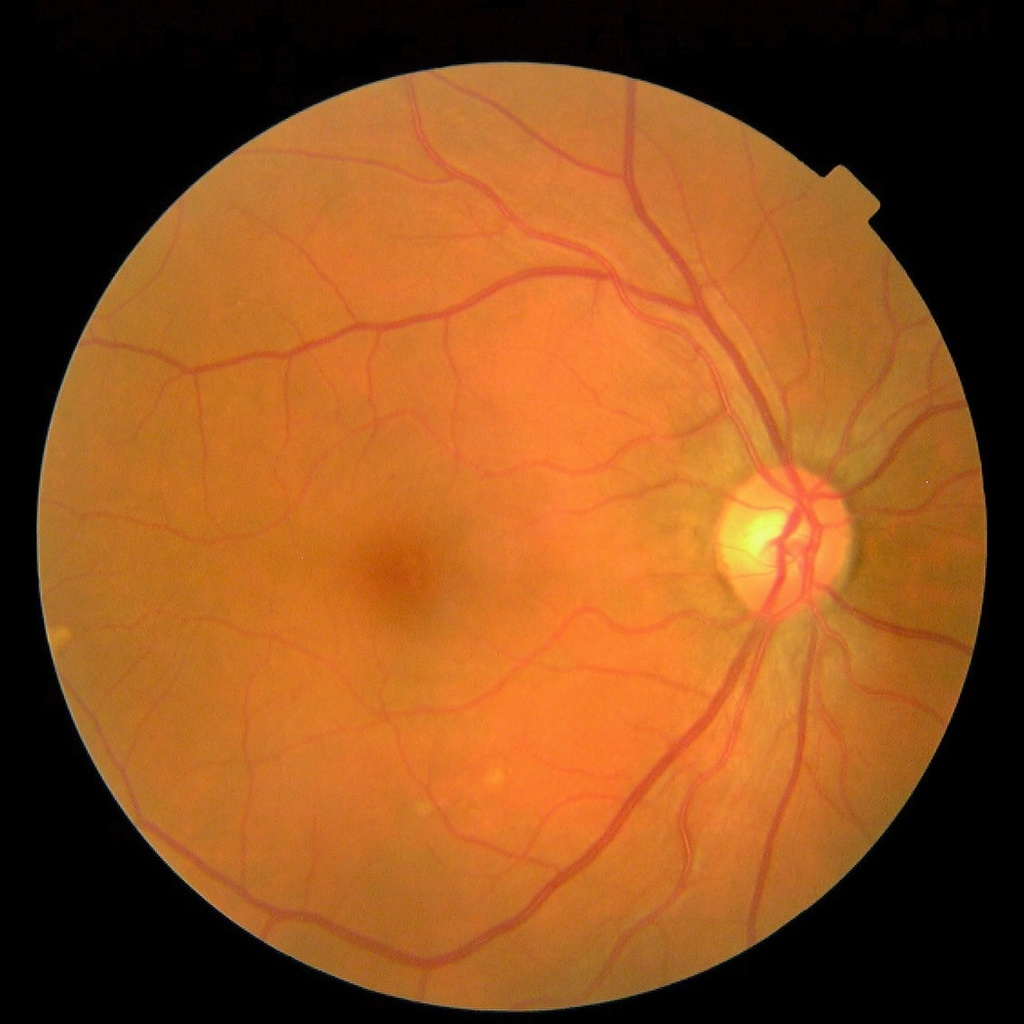
\includegraphics[width=0.2\textwidth]{pics/classified_samples/204_right_1.jpg} &
	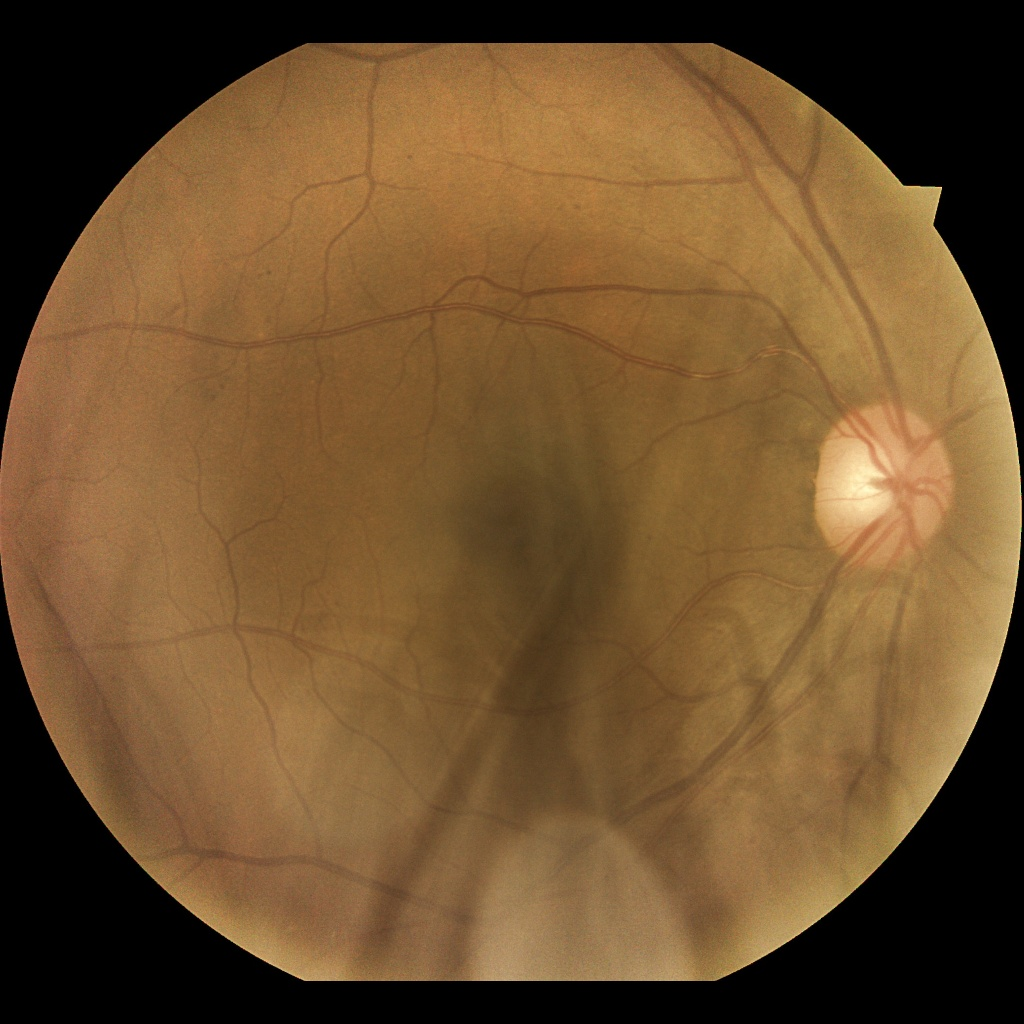
\includegraphics[width=0.2\textwidth]{pics/classified_samples/82_right_2.jpg} &
	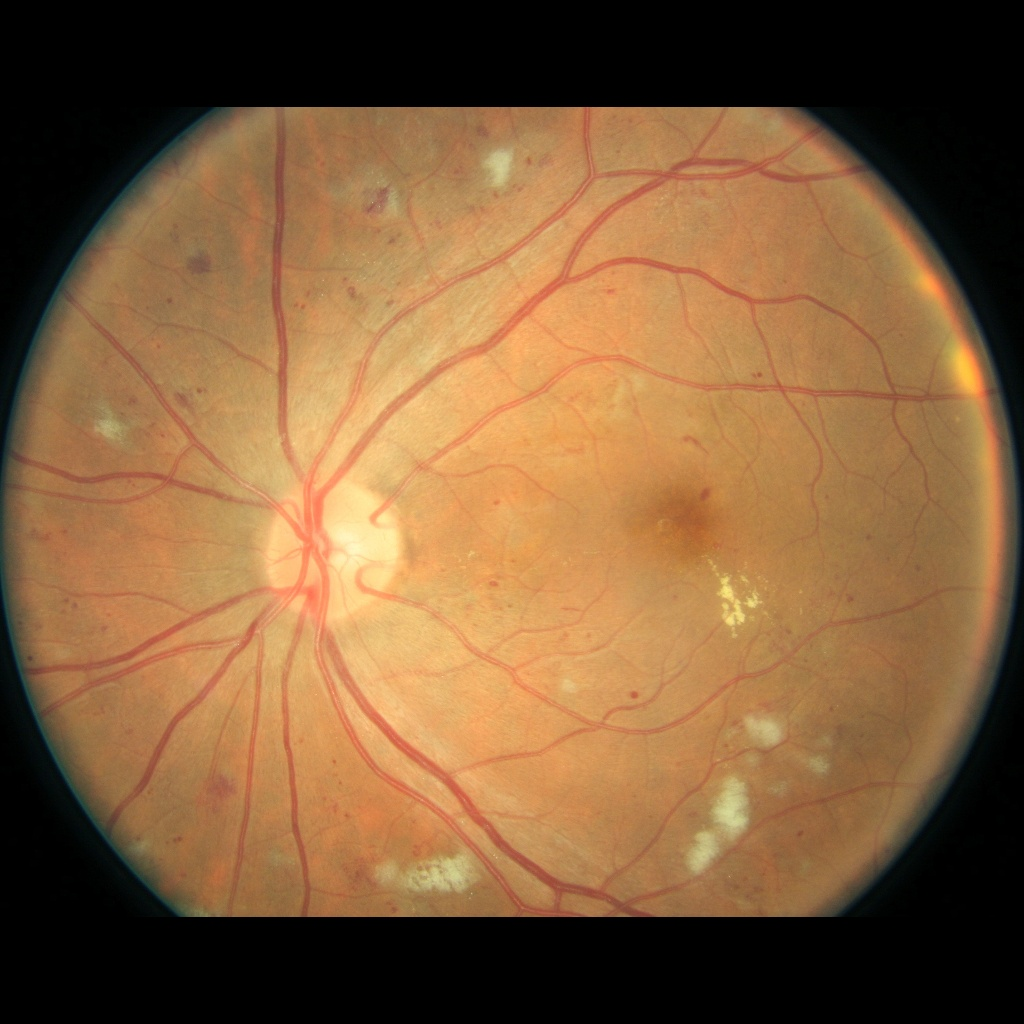
\includegraphics[width=0.2\textwidth]{pics/classified_samples/687_right_3.jpg} &
	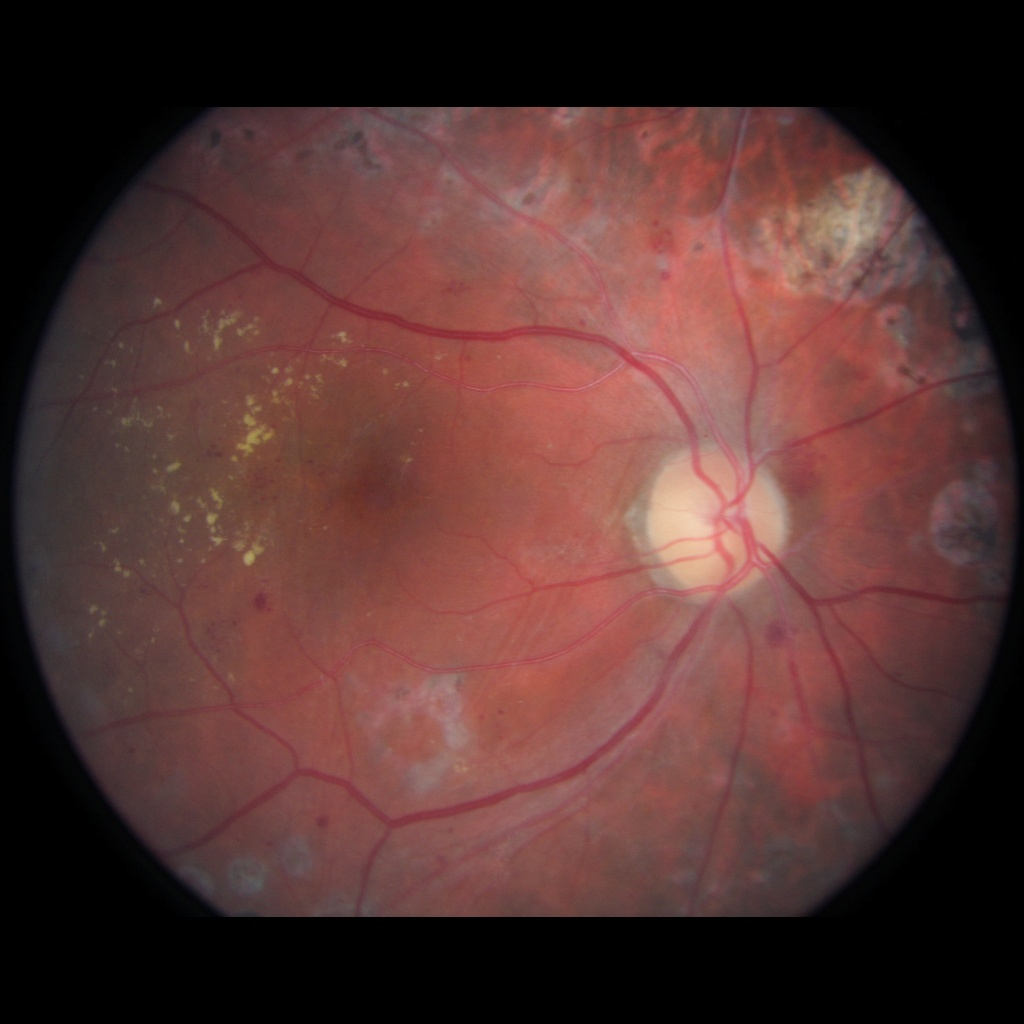
\includegraphics[width=0.2\textwidth]{pics/classified_samples/2496_left_4.jpg} \\\noalign{\vspace{-0.15cm}}
\hline
	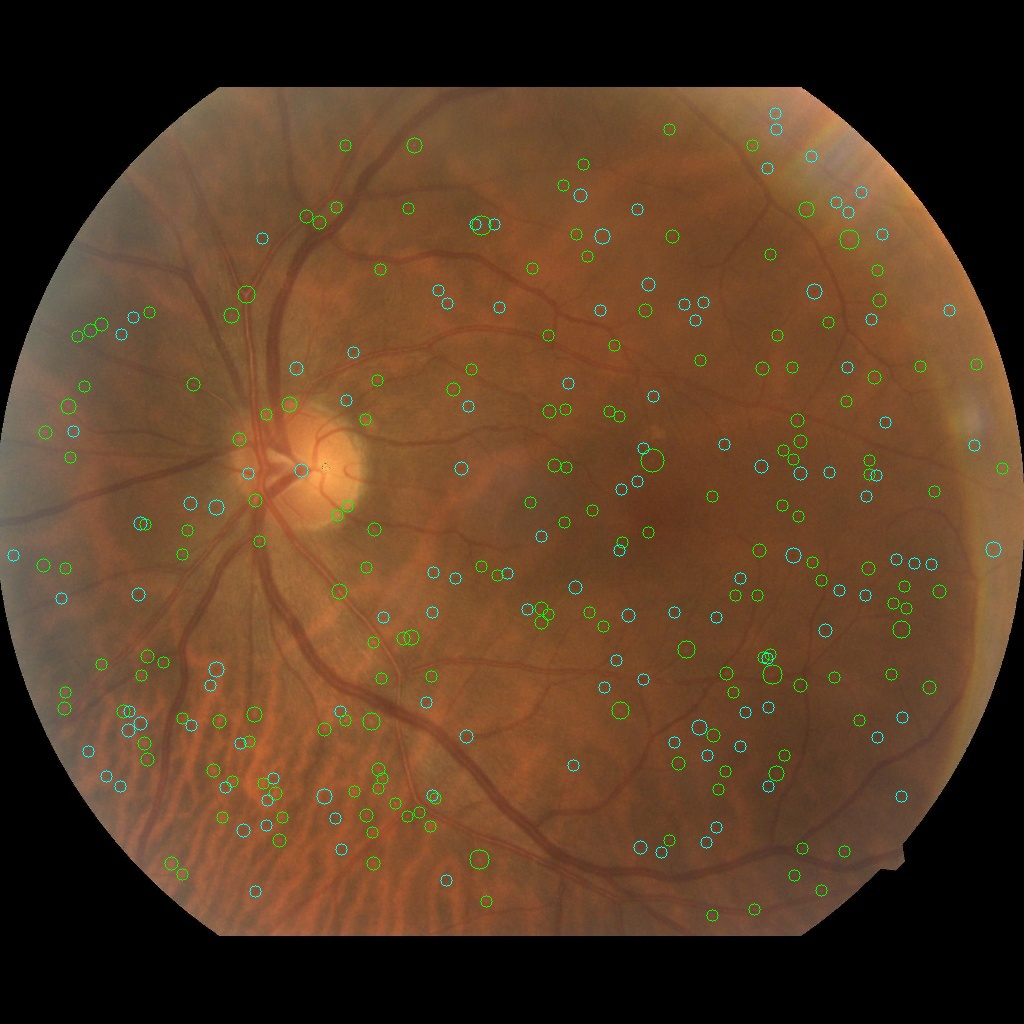
\includegraphics[width=0.2\textwidth]{pics/classified_samples/197_left_0_blobs.jpg} &
	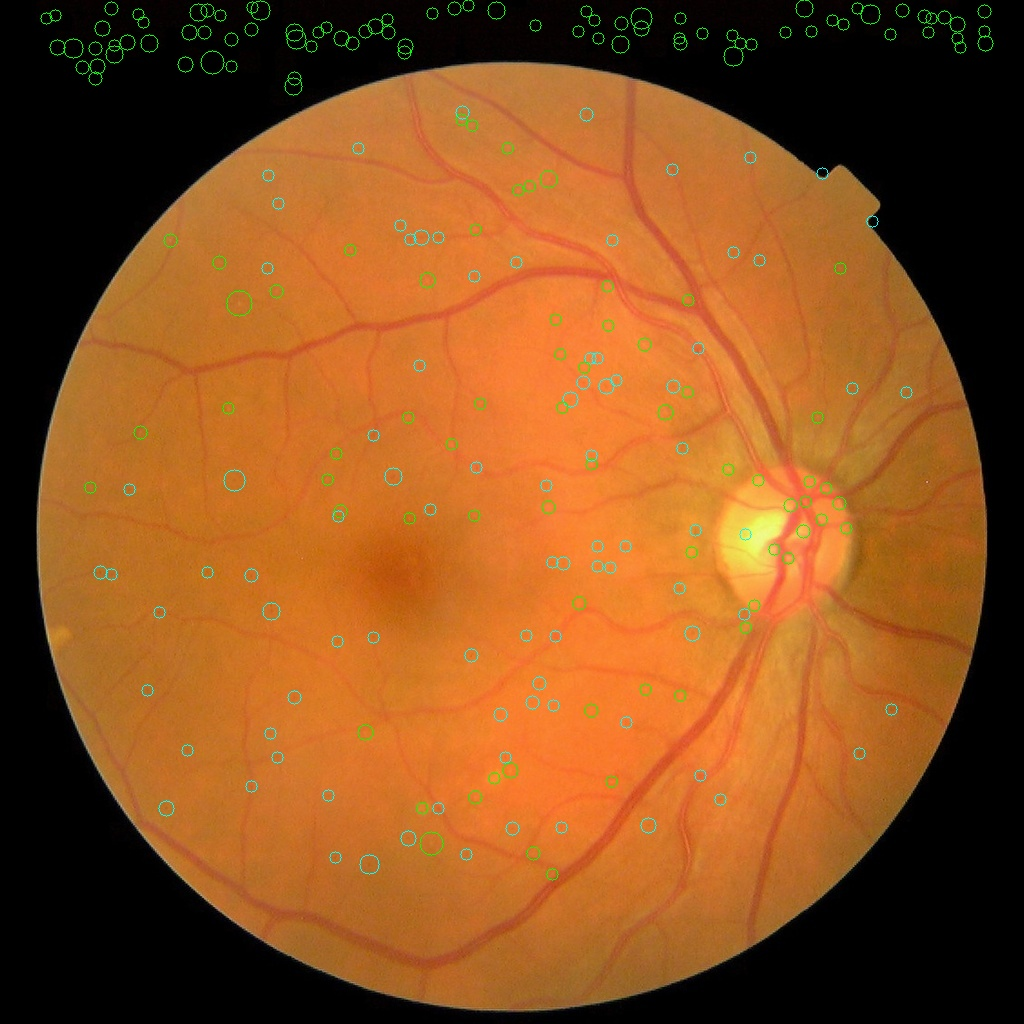
\includegraphics[width=0.2\textwidth]{pics/classified_samples/204_right_1_blobs.jpg} &
	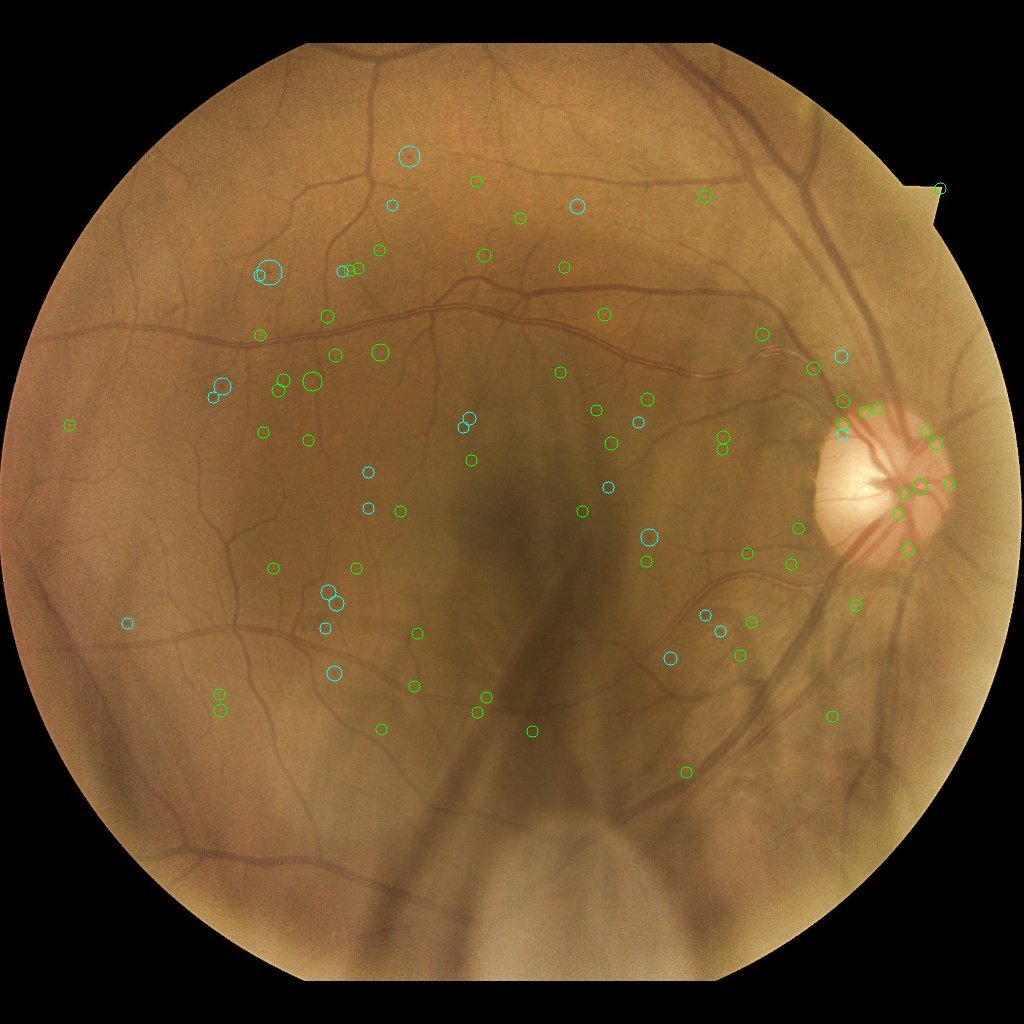
\includegraphics[width=0.2\textwidth]{pics/classified_samples/82_right_2_blobs.jpg} &
	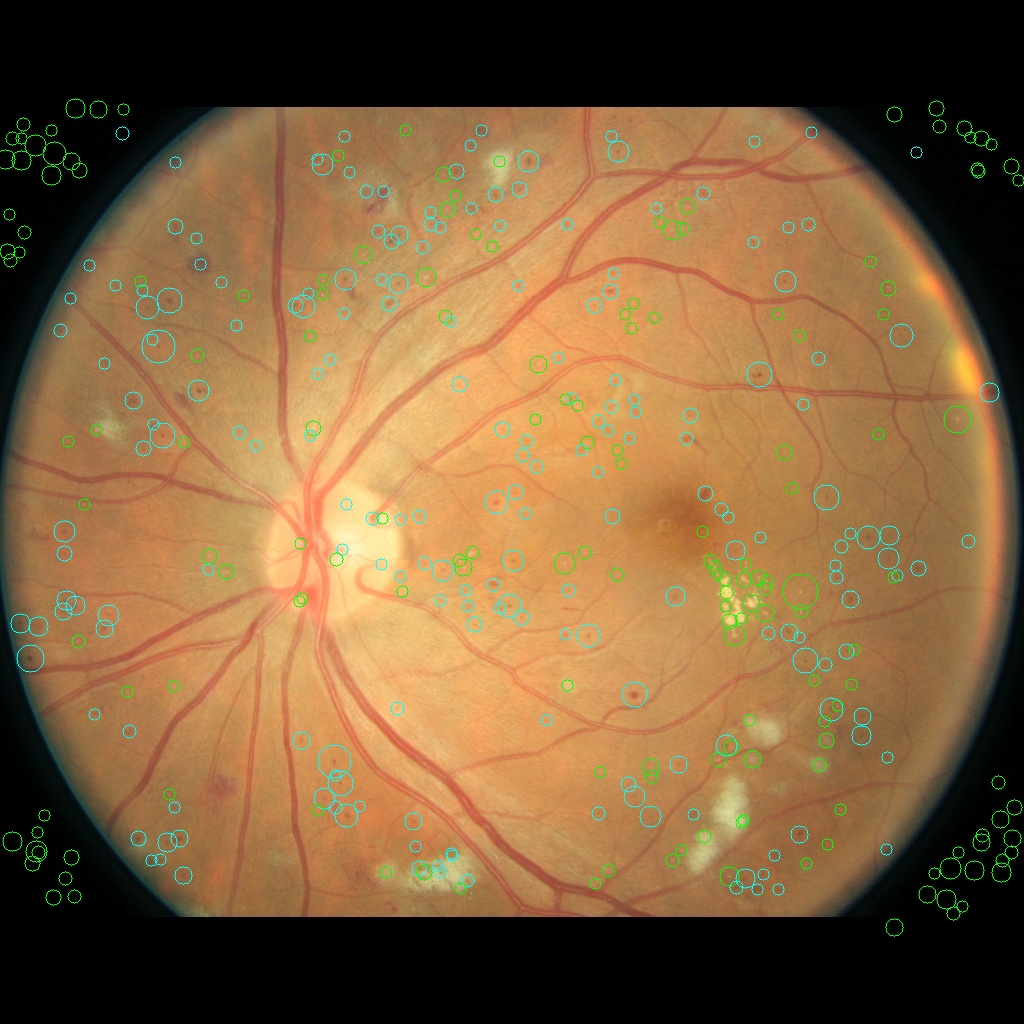
\includegraphics[width=0.2\textwidth]{pics/classified_samples/687_right_3_blobs.jpg} &
	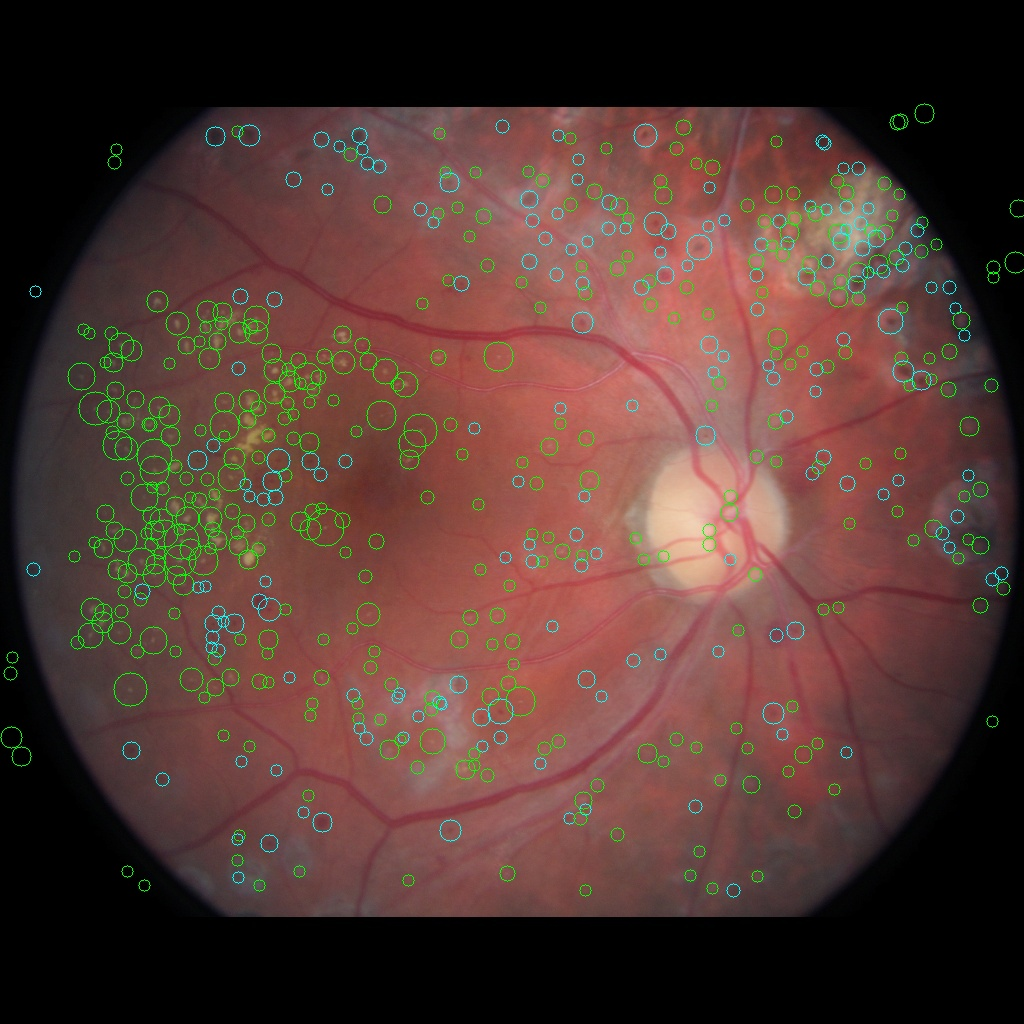
\includegraphics[width=0.2\textwidth]{pics/classified_samples/2496_left_4_blobs.jpg} \\

\end{tabular}
}

\only<2>{
	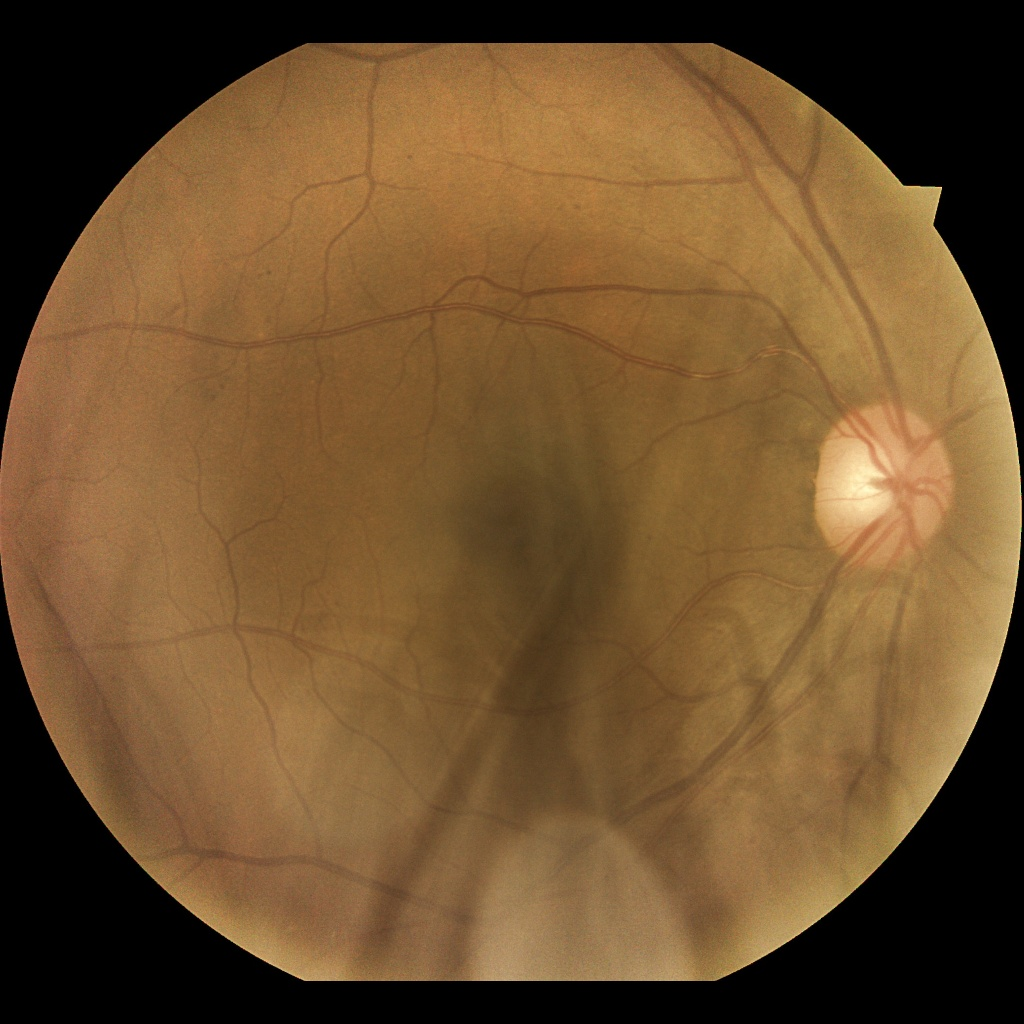
\includegraphics[width=0.65\textwidth]{pics/classified_samples/82_right_2.jpg}
}

\only<3>{
	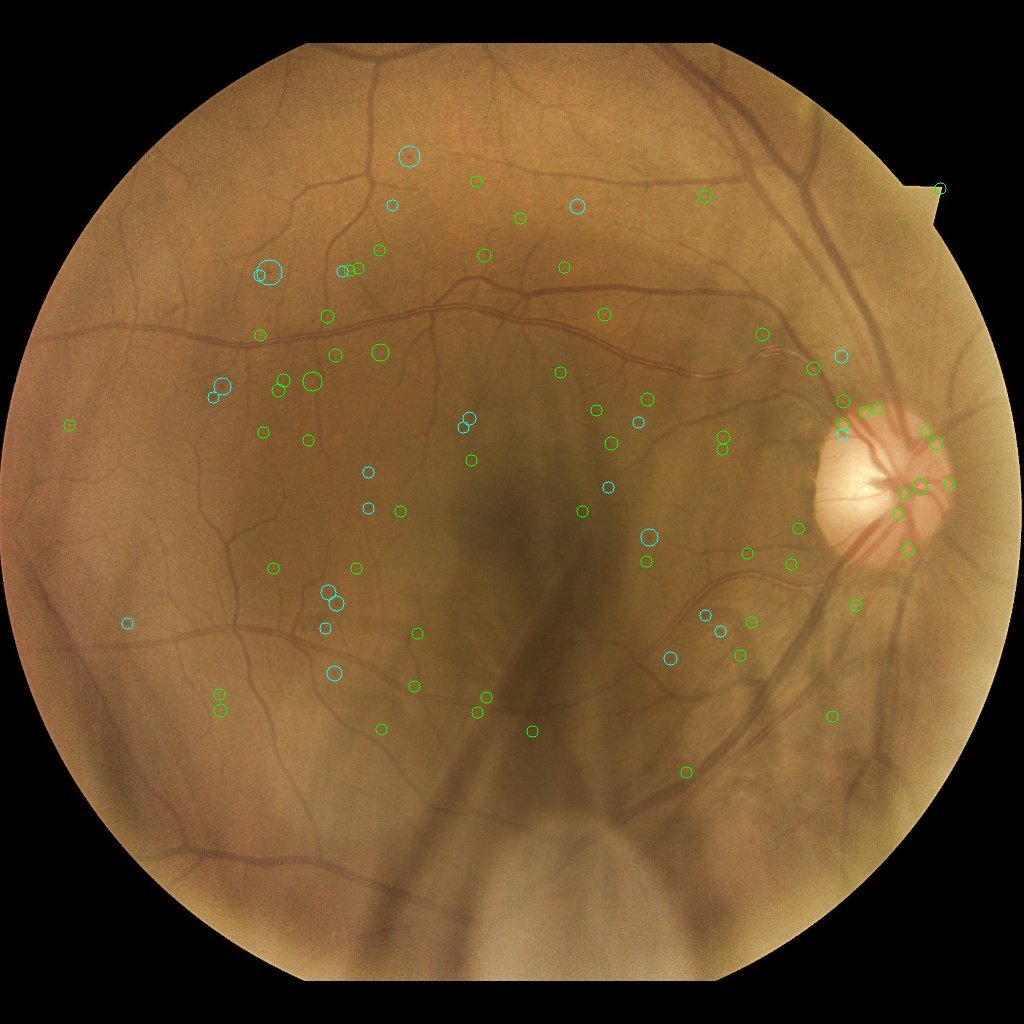
\includegraphics[width=0.65\textwidth]{pics/classified_samples/82_right_2_blobs.jpg}
}
	
\end{frame}

\begin{frame}\frametitle{How blobs looks}

\begin{center}
\begin{tabular}{| b{0.15\linewidth} |@{}c@{}|@{}c@{}|@{}c@{}|@{}c@{}|@{}c@{}|}
\hline
strength & $\sigma = 1.7$ & $\sigma = 3.4$ & $\sigma =  5.1$ & $\sigma = 6.8$ & $\sigma = 8.0$ \\

\hline
$[300,450)$ & 
	\includepatches{patches_300_450_1_2_raw.pdf} & 
	\includepatches{patches_300_450_3_4_raw.pdf} & 
	\includepatches{patches_300_450_5_6_raw.pdf} & 
	\includepatches{patches_300_450_6_7_raw.pdf} & 
	\includepatches{patches_300_450_7_9_raw.pdf} \\

\hline
$[450, 600)$ & 
	\includepatches{patches_450_600_1_2_raw.pdf} & 
	\includepatches{patches_450_600_3_4_raw.pdf} & 
	\includepatches{patches_450_600_5_6_raw.pdf} & 
	\includepatches{patches_450_600_6_7_raw.pdf} & 
	\includepatches{patches_450_600_7_9_raw.pdf} \\
	
\hline
$[600, 750)$ & 
	\includepatches{patches_600_750_1_2_raw.pdf} & 
	\includepatches{patches_600_750_3_4_raw.pdf} & 
	\includepatches{patches_600_750_5_6_raw.pdf} & 
	\includepatches{patches_600_750_6_7_raw.pdf} & 
	\includepatches{patches_600_750_7_9_raw.pdf} \\

\hline
$[750, \infty)$ & 
	\includepatches{patches_750_5000_1_2_raw.pdf} & 
	\includepatches{patches_750_5000_3_4_raw.pdf} & 
	\includepatches{patches_750_5000_5_6_raw.pdf} & 
	\includepatches{patches_750_5000_6_7_raw.pdf} & 
	\\

\hline
\end{tabular}
\end{center}
\end{frame}


\begin{frame}\frametitle{How blobs looks}

\begin{center}
\begin{tabular}{| b{0.15\linewidth} |@{}c@{}|@{}c@{}|@{}c@{}|@{}c@{}|@{}c@{}|}
\hline
strength & $\sigma = 1.7$ & $\sigma = 3.4$ & $\sigma =  5.1$ & $\sigma = 6.8$ & $\sigma = 8.0$ \\

\hline
$[300,450)$ & 
	\includepatches{patches_300_450_1_2_scaled.pdf} & 
	\includepatches{patches_300_450_3_4_scaled.pdf} & 
	\includepatches{patches_300_450_5_6_scaled.pdf} & 
	\includepatches{patches_300_450_6_7_scaled.pdf} & 
	\includepatches{patches_300_450_7_9_scaled.pdf} \\

\hline
$[450, 600)$ & 
	\includepatches{patches_450_600_1_2_scaled.pdf} & 
	\includepatches{patches_450_600_3_4_scaled.pdf} & 
	\includepatches{patches_450_600_5_6_scaled.pdf} & 
	\includepatches{patches_450_600_6_7_scaled.pdf} & 
	\includepatches{patches_450_600_7_9_scaled.pdf} \\
	
\hline
$[600, 750)$ & 
	\includepatches{patches_600_750_1_2_scaled.pdf} & 
	\includepatches{patches_600_750_3_4_scaled.pdf} & 
	\includepatches{patches_600_750_5_6_scaled.pdf} & 
	\includepatches{patches_600_750_6_7_scaled.pdf} & 
	\includepatches{patches_600_750_7_9_scaled.pdf} \\

\hline
$[750, \infty)$ & 
	\includepatches{patches_750_5000_1_2_scaled.pdf} & 
	\includepatches{patches_750_5000_3_4_scaled.pdf} & 
	\includepatches{patches_750_5000_5_6_scaled.pdf} & 
	\includepatches{patches_750_5000_6_7_scaled.pdf} & 
	\\

\hline
\end{tabular}
\end{center}
\end{frame}

\subsection{Bag of visual words}
\begin{frame}\frametitle{BoVW preparation}
\begin{itemize}
\item Extract local descriptors from blob patch: HOG, LBP
\item K-means segmentation for quantization
\item Use histograms of visual words as feature vectors
\end{itemize}
\end{frame}

\begin{frame}\frametitle{BoVW preparation}
\par Unfortunately I got stuck on this point two weeks before challenge deadline. :-(
\begin{center}
\begin{figure}
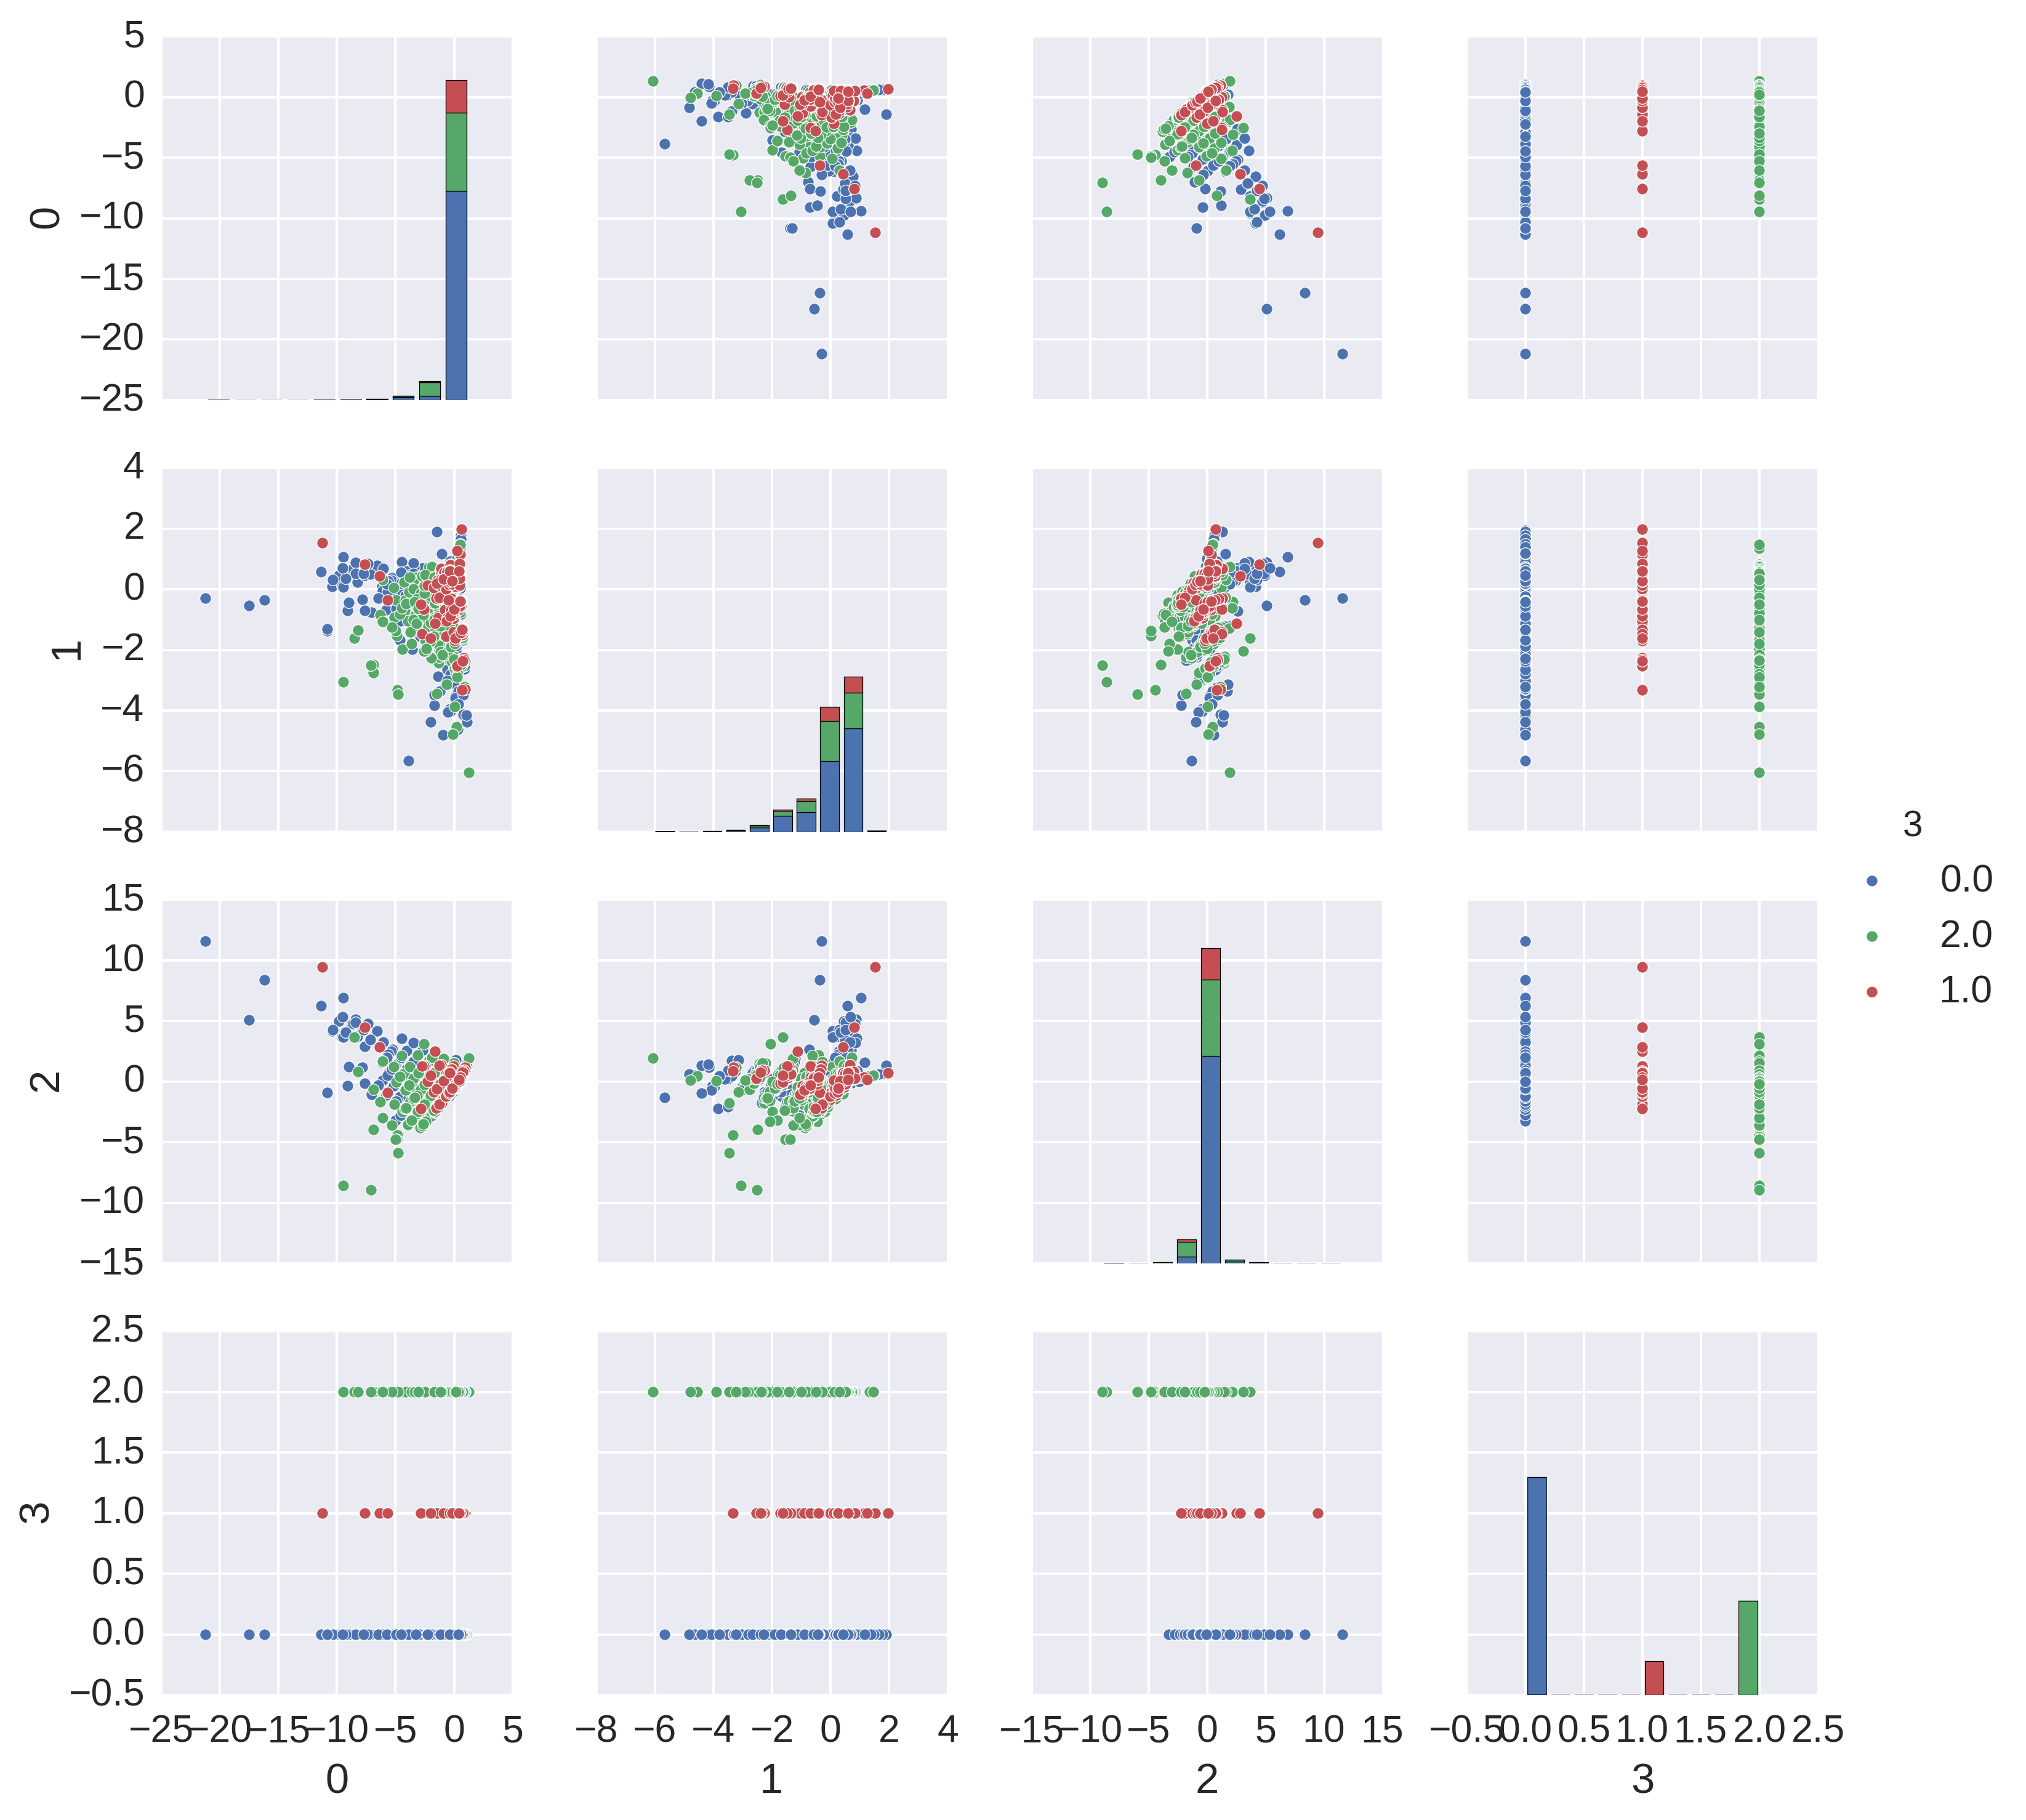
\includegraphics[width=0.5\textwidth]{pics/bow_pca_results.png}
\caption{Typical picture of BoW features  after applying PCA.}
\end{figure}
\end{center}
\end{frame}